\documentclass {article}
\usepackage{enumitem}
\usepackage{listings}
\usepackage{float}
\usepackage{mathtools}
\usepackage{graphicx}
\graphicspath{ {images/} }

\renewcommand*\rmdefault{cmr}

\lstset{ %set options for lstlisting = codesnippets
	breaklines=true, 
	captionpos=b,
	keepspaces=true,
	numbers=left,
	tabsize=2
}

\title{A comparison between functional and object oriented programming approaches in JavaScript}
\date{now}
\author{
Kim Svensson Sand
Tord Eliasson
}

\begin{document}
\maketitle
\pagenumbering{gobble}
\newpage
\pagenumbering{arabic}
\section{Abbreviations}
\begin{itemize}[leftmargin=*]
\item [ ] ECMAScript 2015 = ES6
\item [ ] Functional Programming = FP
\item [ ] Object-Oriented Programming = OOP
\end{itemize}
\section{Background and Related work}
Object oriented or imperative languages are dominating with languages such as C, C++, Java and C\#, however functional languages seem to be gaining in popularity for handling big data and concurrency with languages such as Scala, Erlang or Haskell [1, 4, 9, 11]. Some are also arguing that a more functional approach will give you less code, more readable code, code that is easier to maintain and easier to test, and that learning it will give you better experience as a programmer [1, 2, 3, 9].

Here we will describe the functional programming paradigm, FP, and also the object oriented programming paradigm, OOP. 
\subsection{Functional programming}
Functional programming, FP, is a programming paradigm that at its core is based on lambda-calculus [35]. Programs are constructed using functions and by avoiding changing the state. By not modifying the state side effects are avoided. Computation is done by changing the environment, rewriting the functions, rather than changing variables. Multiple functions can be composed into larger and more complex functions, and should be reduced to its simplest state following mathematical rules. The following are concepts used in FP.
\begin{description}
\item [Lazy evaluation] - Lazy evaluation is when a value is not calculated until it is needed [5].
\item [Static type checking] - Pure functional languages usually have static type checking [35]. This means that variables are of a certain type, for example int or char. In such languages it is not allowed to use functions with the wrong types. So if there is for example a function taking an int as parameter it is illegal to call that function with a String as its parameter. In dynamic type checked-languages this would be legal, since variables are not specified as types, and might cause an unexpected error. For example we can use JavaScript:

\begin{lstlisting}[language=Java]
//JavaScript has dynamic type checking
function double(nr) {
return nr * 2;
}

var word = "string";
double(word); //Will return NaN but still continue running
\end{lstlisting}

\item [ ] A similar program in golang, that is a statically type checked language:

\begin{lstlisting}[language=Java]
func main() {
  var word string = "string"
  fmt.Printf("%d", double(word)) //Error: cannot use word (type string) as type int in argument to double
}

func double(nr int) int {
  return nr * 2
}
\end{lstlisting}

\item [ ] will give an error when compiling.
\item [Side effects] - Side effects are for example changing a variable or any interaction outside the function [1]. This is avoided in functional programming since it may result in incorrect and unexpected behaviour. 
\item [Pure functions] - A pure functions always returns the same result, given the same input, and does not have side effects [1]. See the following example. 

\begin{lstlisting}[language=Java]
var sum = 0;

//Impure
function add(a, b) {
  sum = a + b;
}

//Pure
function add(a, b) {
  var tmp = a + b;
  return tmp;
}
\end{lstlisting}

\item [Higher order functions] - Higher order functions are an important concept in functional programming [5]. First class functions mean that functions are treated as values, which means that they can be stored in variables, stored in arrays or created if needed. A higher order function is a first class function that either takes a function as a parameter, returns a function as a result or both. This makes it possible to compose larger and more complex functions.

\begin{lstlisting}[language=Java, breaklines=true]
function add(a, b) {
  return a + b;
}

//Functions can be placed in variables.
var thisFunc = add;

//And also put in other variables.
var sameFunc = thisFunc;
sameFunc(1, 2); //Will give the output 3.

//Functions can also be used as parameters or return values.
function applyFunc(f, a, b) {
  return f(a, b);
}

applyFunc(function(a, b) {
  return a * b;
}, 3, 2); //Will give output of 6

//Returns a function that returns a string
function getStringCreator(category, unit) {
  return function(value) {
    return category + ': ' + value + unit;
  }
}

var weightStringCreator = getStringCreator('Weight', 'kg');
weightStringCreator(5); //Outputs “Weight: 5kg”
\end{lstlisting}

\item [Recursion] - Recursive functions are functions that call themselves and are used as loops [5]. It is important in functional programming since it can hide mutable state and also implement laziness. In functional programming recursion is used rather than loops.

\begin{lstlisting}[language=Java]
//Adds all numbers from start to end with a loop
function iterativeAdd(start, end) {
  var sum = 0;
  while(start <= end) {
    sum += start;
    start++;
  }

  return sum;
}

//Adds all numbers from start to end recursively
function recursiveAdd(start, end) {
  if (start == end) {
    return end;
  }
  else {
    return start + recursiveAdd(start + 1, end);
  }
}
iterativeAdd(1, 6); //Outputs 21
recursiveAdd(1, 6); //Also outputs 21
\end{lstlisting}

\item [Currying] - Currying means a function can be called with fewer arguments than it expects and it will return a function that takes the remaining arguments [1]. 

\begin{lstlisting}[language=Java, breaklines=true]
//Returns a new function that takes the remaining argument or the sum of a and b if both are provided.
function addWithCurrying(a, b) {
  if(b) {
    return a + b;
  }
  else {
    return function(b) {
      return a + b;
    }
  }
}

var curryAdd = addWithCurrying(4); 
curryAdd(6); //Outputs 10
addWithCurrying(4, 6); //Also outputs 10
\end{lstlisting}

\item [Immutable data structures] - In functional programming mutations, that are side effects, are avoided [5]. Hidden side effects can result in a chains of unpredicted behaviour in large systems. Instead of mutating the data itself a local copy is mutated and returned as a result, as seen in the pure functions example.
\end{description}
\subsection{Object oriented programming}
Object oriented programming is a programming paradigm which is built around “objects”. These objects may contain data, in form of fields, often referred as attributes and code in form of procedures, often referred to as methods [26].

These objects are created by the programmer to represent something with the help of its attributes and methods. For example, a class can represent an employee. An employee has the attributes assignment and salary. The employee also has a method for doing work. Then the employee has to work somewhere, so we create another object for a company where our employee can work. The company has the attributes income and number of employees. It also has methods to hire employees and fire employees. Since there are more employees who works at this company, we can add more employees by creating new objects of the information in employee class.

By building objects together like this, you can build programs by the object oriented paradigm.  

\begin{description}
\item [Class] - A class is a model for a set of objects [35]. It establishes what data and functions the object will contain and what names, signature and visibility everything will get in the class. The class also contains the implementation of the functions. Every object belongs to at least one class.

\item [] A class is a model for a set of objects, which clearly the object oriented paradigm is built around[35]. The class establishes what the object will contain, for example variables and functions, and signatures and visibility of these. To create a object of any kind, a class must be present. 

\begin{lstlisting}[language=Java]
//Creates a class Animal with the properties name and age and a function for logging the properties to the screen
class Animal {
  constructor (name, age) {
    this.name = name;
    this.age = age;
  }

  logAnimal() {
    console.log('Name: ' + this.name + '\nAge: ' + this.age);
  }
}

var animal = new Animal('Buster', '9');
animal.logAnimal();
//Outputs Name: Buster
//Age: 9
\end{lstlisting}

\item [Object] - An object is a capsule that contains both data and functions that manipulates the data [35]. The data and the functions are accessible from the outside through the object. 
An object is an capsule that contains the variables and functions established in the class. All data and functions can be accessible from outside the object.
\item [Inheritance] - When an object acquire all properties and functionality of another object [41], it is called inheritance. This provides code reusability. 

\begin{lstlisting}[language=Java, breaklines=true]
//Based upon the Animal class with an added property race
//The original logAnimal() is overidden so the new property is also logged to the screen.
class Dog extends Animal {
  constructor(name, age, race) {
    super(name, age);
    this.race = race;
  }

  logAnimal() {
    super.logAnimal();
    console.log('Race: ' + this.race);
  }
}

var dog = new Dog('Buster', '9', 'Shitzu');
dog.logAnimal();
//Outputs Name: Buster
//Age: 9
//Race: Shitzu
\end{lstlisting}

\item [Encapsulation] - Encapsulation can be used to refer to two different things [35, 41]. A mechanism to restrict direct access to some object components and the language construct that facilitates the bundling of data with methods. The access part is done by making the different parts of an object public or private and the bundling is made with objects.
\end{description}
\subsection{JavaScript}
But how does the support for the different paradigms in JavaScript look?
\subsubsection{Functional programming}
JavaScript is not a functional language, but it is possible to write functional code with it [1]. There are also libraries that makes functional programming in JavaScript easier, such as Underscore.js [5], however we will use ECMA 2015, ES6, that already provide many of the functions provided by Underscore.js. This is also to use similar environment for our different implementations in this experiment.

In JavaScript it is possible to treat functions as any other variable, pass them as function parameters or store them in arrays, so called first class functions [1]. There are also higher order functions such as map(), filter() and reduce() that might replace loops [2]:

\begin{description}
\item [map()] - Takes calls a provided function on every element in an array and returns an array with the outputs [27].
\item [filter()] - Returns a new array with all the elements that passes a test in a provided function. 
\item [reduce()] - Reduces a array to a single value.
\end{description}

However there is no automatic currying in JavaScript. If currying is needed, it has to be implemented manually.
\subsubsection{Object oriented programming}
JavaScript has always had support for OOP. But 
with the new version of JavaScript, called ECMAScript 2015 or ES6, OOP starts to look more like classical OOP languages like for example Java [30].

JavaScript supports all of the concepts mentioned above [30].
\subsection{Related work}
In “Curse of the excluded middle” [3] Erik Meijer arguments with multiple examples that the industry should not focus on a combination between functional and objected oriented methods to counter handling big data with concurrency and parallelism. He concludes that it is not good enough avoid side effects in imperative or object oriented languages. It is also not good enough to try to ignore side effects in pure functional languages. Instead he thinks that people should either accept side effects or think more seriously about using the functional paradigm.

In “Functional at scale” [4] by Marius Eriksen he is explaining why Twitter uses methods from functional programming to handle concurrent events that arises in large distributed systems in cloud environments. In functional programming it is possible build complex parts out of simple building blocks, thus making systems more modular. He concludes that the functional paradigm has multiple tools for handling the complexity present in modern software.

Eriksson and Ärleryd are looking at how to use functional practises when developing front end applications by taking inspiration from Elm in their master's thesis [11]. They have researched each practise in Elm to see if it is possible to use these practises in JavaScript together with tools and libraries. Their conclusion was that it is possible to replicate functional practises from Elm in JavaScript, but that they prefer working with Elm. In JavaScript multiple libraries would have to be used to use the same practises. They also concluded that even though functional programming is not widely used within the industry, functional practises can still be used in all projects.

In “Improving Testability and Reuse by Transitioning to Functional Programming” [12], Benton and Radziwill state that functional programming is better suited for test driven development (TDD) and concludes that a shift toward the functional paradigm benefits reuse and testability of cloud-based applications.

Alic, Omanovic and Giedrimas has made a comparative analysis of functional and object-oriented programming languages[15]. They have compared four languages, C\#, F\#, Java and Haskell based on performance, runtime and memory usage. Their conclusion is that Java is the fastest while Haskell uses much less memory, and that programming paradigms should be combined to increase execution efficiency. 

Dobre and Xhafa writes in “Parallel Programming Paradigms and Frameworks in Big Data Era” that we now are in a big data era[47]. They also review different frameworks, programming paradigms and more in a big data perspective. Around paradigms they state, “functional programming (FP) is actually considered today to be the most prominent Programming Paradigm, as it allows actually more flexibility in defining Big Data distributed processing workflows.”

Mention concurrency, scala osv? Argument why this subject might be relevant. Functional programming can give more experience, more popular in the industry blablabla. Find studies!
\section{Method}
What we are doin’.
\subsection{Algorithms}
In this experiment we will implement four different algorithms. We have chosen algorithms that are well known, so that our focus will be on the different implementations, rather than on how the algorithms work. 
We will implement a search tree, the shellsort algorithm, the tower of hanoi algorithm and Dijkstra’s algorithm. In the search tree we will implement tree traversal,  which is a recursive algorithm, as is the tower of hanoi algorithm. These algorithms fit well for FP since it uses recursion. The implementation of the binary tree structure can however be implemented by using classes and objects, that is used in OOP. Shellsort uses state and iteration which is used in OOP and avoided in FP. Dijkstra’s algorithm also uses state and iteration, and the graph can also be implemented using classes and objects.

We chose algorithms that uses both recursion and iteration to not give advantage to any paradigm. When implementing these algorithms and data structures we can also make use of OOP methods, such as classes and objects. The algorithms purpose are also different to avoid for example implementing four different sorting algorithms. 
\subsubsection{Tree search algorithms}
A binary tree is a tree consisting of nodes, where a node can have a maximum of two children [38]. These children can be described as the left and the right subtree and the parent is the root. The property that differs a binary search tree from a standard binary tree, is the order of the nodes. In a binary tree the order can be undecided, but in a search tree the nodes are stored in an order based on some property. For example in our binary search tree the left subtree of a root will contain smaller numbers than the root, and the right subtree will contain larger numbers. Using tree traversal it is possible to find certain nodes or get a list of sorted objects. Our binary tree will contain random numbers and the functions:
\begin{description}
\item [findNode(comparable, rootNode)] - Finds a specific key in the tree.
\item [inOrderTraversal(root)] - Returns an array of all numbers in the tree, sorted smallest to biggest.
\item [insert(comparable, rootNode)] - Inserts number into the tree. Returns true or false depending on success. If comparable is already in the tree, false should be returned. Note that in the functional implementation this function will return the resulting tree instead of mutating the tree and returning true or false.
\end{description}

\begin{figure}[H]
\includegraphics[width=\textwidth]{binary-tree-example}


\caption {Binary tree example}
\end {figure}

\begin{description}
\item[Algorithm descriptions in psudocode]
\item[]
\item [findNode(comparable, root)]
\item[]
\begin{lstlisting}[language=Pascal]
if comparable is equal to comparable in root then
 	return root
else if comparable is larger than comparable in root then
 	return findNode(comparable, rightSubtree in root)
else if comparable is smaller than comparable in root then
 	return findNode(comparable, leftSubtree in root)
end if
\end{lstlisting}

\item [algorithm inOrderTraversal(root)]
\item []
\begin{lstlisting}[language=Pascal]
set array to empty array
if comparable in root is undefined then
 	return array
else if comparable in root is not undefined then
 	add inOrderTraversal(leftSubtree in root) to end of array
 	add comparable in root at end of array
 	add inOrderTraversal(rightSubtree in root) at end of array
 	return array
end if
\end{lstlisting}

\item[] Running this in the tree in Figure1 would return the array [8, 10, 15, 18, 24, 22, 31, 39, 48, 52, 56, 71, 84, 88, 90, 93].

\item [insert(comparable, root)]
\item []
\begin{lstlisting}[language=Pascal]
if comparable is equal to comparable in root then
  	return false
else if comparable is larger than comparable in root then
	if rightSubtree in root is undefined
		create newNode
		set comparable in newNode to comparable
		set rightSubtree of root to newNode
		return true
	else if rightSubtree in root is not undefined then
  		return insert(comparable, rightSubtree in root)
 	end if
else if comparable is smaller than comparable in root then 
 	if leftSubtree in root is undefined then 
create newNode
 		set comparable in newNode to comparable
 		set leftSubtree in root to newNode
 		return true
 	else if leftSubtree in root is not undefined then
 		return insert(comparable, leftSubtree in root)
 	end if
end if
\end{lstlisting}
\end{description}
\subsubsection{Shellsort algorithm}
The shellsort algorithm is named after its creator Donald Shell [13]. It was one of the first algorithms to break the quadratic time barrier. The algorithm sorts by sorting items using insertion sort with a gap. For each run the gap is decreased until the gap is 1 and the items are sorted. How the gap is decreased is decided with a gap sequence. Different gap sequences gives shellsort a different worst-case running time.
 
We will use one of Sedgewick’s gap sequences that has one of the fastest worst-case running times \(O(n^3/4)\). 

The sequence is 

\(\{1, 5, 19, 41, 109\}\), where the terms are of the form

\(4^k - 3 * 2^k + 1\), or

\(9 * 4^k - 9 * 2^k + 1\)
 
In our implementation the sequence is put in an array and not calculated during execution, since we do not want to get different results between our implementation because of the calculation of the gap sequence.

This algorithm will sort an array filled with randomized numbers. Our implementation uses this algorithm in a function:

\begin{description}
\item[shellsort(array)] - Takes an unsorted array as an input and returns a sorted copy of the array.

\item[algorithm shellsort(array of size n)]
\item []
\begin{lstlisting}[language=Pascal]
set sortedArray to array
set gapSequence to Sedgewick’s gap sequence.
set currentGapIndex to 0
set currentGap to the largest gap i gapSequence where gap is smaller than n divided by 2
set currentGapIndex to the index of currentGap in gapSequence
while currentGap is larger than 0 do
 	for i = currentGap to n
 		set currentValue to array[i]
 		set currentIndex to i
 		while currentIndex - currentGap is larger or equal to 0 and sortedArray[currentIndex - currentGap] is larger than currentValue do
 			set sortedArray[currentIndex] to sortedArray[currentIndex - currentGap]
 			set currentIndex to currentIndex - currentGap
 		end while
 		set sortedArray[currentIndex] to currentValue
 	end for
 	set currentGapIndex to currentGapIndex - 1
 	set currentGap to gapSequence[currentGapIndex]
end while
return sortedArray
\end{lstlisting}
\end{description}
\subsubsection{The Tower of Hanoi algorithm}
The Tower of Hanoi is a game invented by mathematician Édouard Lucas in 1883 [14]. The game consists of three pegs and a number of disks stacked in decreasing order on one of the pegs. The goal is to move the tower from one peg to another by moving one disk at a the time to one of the other pegs. A disk can not be placed on a peg on top a smaller disk. 

\begin{figure}[H]
\includegraphics[width=\textwidth]{tower-of-hanoi-example}

\caption{Tower of hanoi image}
\end{figure}

This algorithm will move a tower from one peg to another in the function:

\begin{description}
\item[hanoi(tower, start, dest, aux)] - Moves tower from start to dest following the rules of the tower of hanoi problem. Returns the start, dest and aux pegs with the repositioned tower.


\item[Algorithm description:]
\item[] Pseudo code based on that tower is the number of the largest disk, where 0 is the smallest disk in the tower.
\begin{lstlisting}[language=Pascal]
if tower is equal to 0
 	move tower from start to dest
else
 	hanoi(tower - 1, start, aux, dest)
 	move tower from start to dest
 	hanoi(tower - 1, aux, dest, start)
end if
\end{lstlisting}
\end{description}
\subsubsection{Dijkstra’s algorithm}
Dijkstra’s algorithm is an algorithm for finding the shortest path in a graph consisting of a number of nodes connected by edges [18], where the weight of the edges is known. The algorithm will find the shortest path from the start node to the end node in a graph. It is initiated by:
\begin{enumerate}
\item setting the distance to the start node to 0.
\item setting the distance to all other nodes to infinity.
\item mark all nodes as unvisited.
\end{enumerate}
The algorithm will then find the shortest path using the following steps:
\begin{enumerate}
\item Set current node to the node with the smallest distance that has not already been visited.
\item For all neighbors to current node that has not already been visited, check if their distance is smaller than the distance of current node + the distance to the neighbor. If so, update the distance of the neighbor.
\item Mark current node as visited.
\item Repeat until all nodes have been visited or the end node has been visited.
\end{enumerate}

\begin{figure}[H]
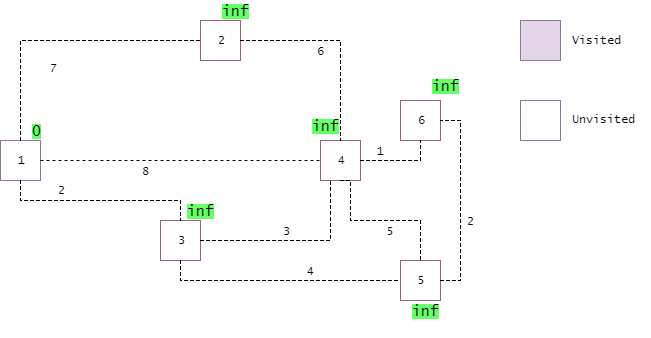
\includegraphics[width=\textwidth]{dijkstras-algorithm-example1}

\caption{After initiation of Dijkstra’s algorithm}
\end{figure}
\begin{figure}[H]
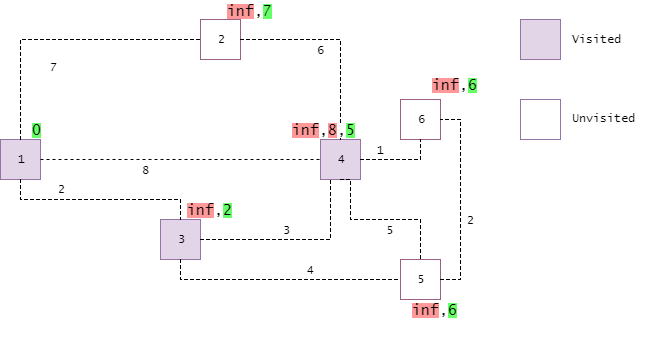
\includegraphics[width=\textwidth]{dijkstras-algorithm-example2}

\caption{After three nodes have been visited with Dijkstra’s algorithm}
\end{figure}

This algorithm will be used in a function:
\begin{description}
\item[dijkstras(graph, startNode, endNode)] - That takes graph, startNode and endNode and returns an array with the shortest path from startNode to destNode. 

\item [Algorithm description:]
\item[]
\begin{lstlisting}[language=Pascal]
for each node in graph
 	set dist[node] to infinity 
 	set path[node] to undefined 
end for
set dist[startNode] to 0 
set unvisitedNodes to nodes in graph
while unvisitedNodes is not empty or endNode is not in unvisitedNodes do
 	set current to node where dist[node] is smallest and node is in unvisitedNodes
 	remove current from unvisitedNodes
  	for each neighbor of current where neighbor is in unvisited do
    		set temp to dist[current] + weight of edge in graph, where edge is from current to neighbor distance between current and neighbor node
 		if temp is smaller than dist[neighbor] then
 			set dist[neighbor] to temp
 			set path[neighbor] to path[current] + current
 		end if
 	end for
end while
return path[endNode]
\end{lstlisting}
\end{description}
\subsection{Testing}
Our code will be tested through code reviews and unit testing.
\subsubsection {Code reviews}
We will review each other’s implementations and our implementations will also be reviewed by a third party. The reviews should help us to find bugs and also to confirm that we have used FP or OOP methods.
\subsubsection{Unit testing}
Unit testing will be done using the JavaScript libraries Mocha [45] for writing tests, Chai [46] for evaluating expressions, and Karma [44] for automated tests.

Our implementations will have to pass the tests in AppendixA to be accepted as done.
\subsubsection{Rules for paradigms}
\subsection{Implementation}
JavaScript does not have a strong or static type system, so we will use Flow, that is a static type checker for JavaScript [40]. It allows typing of variables, checks the code for bugs and translates into pure JavaScript.  

\section{Appendices}
Put test table here

Input tree


Output tree



Input graph

Output graph
\end{document}
